\section{Research}
\label{r:stuff}

\subsection{Design overview}
\label{s:design}
%
%When a user lands on an advertiser's website, the advertiser wants two pieces of information: (1) is this a real human, or a sybil? and (2) which ad was effective at sending this user here?
%
%In case this is a real user, the advertiser needs to reward the publisher/platform who showed the ad to the user.
%
%In case the user makes a purchase, the advertiser needs to pay the platform, which rewards the publisher for the success of the ad.
%

\begin{figure}
 \centering
 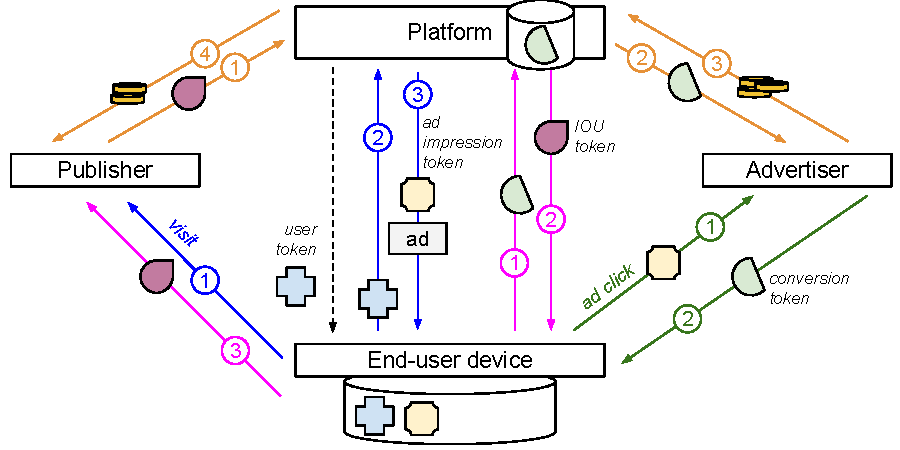
\includegraphics{figures/overview.pdf}
 \caption{Overview of our privacy-preserving ad economy design.}
 \label{f:overview}
\end{figure}

%
We now sketch our privacy-preserving ad ecosystem in which the cryptographic protocols combined with the participants' incentives prevent them from cheating (Figure~\ref{f:overview}).
%

%
The platform (\eg Google or Meta) has a notion of active, non-sybil users, established \eg by continued engagement on the platform's services and a plausible usage history that is costly to fake.
%
For each such user, the platform issues their devices with a secret that the browser on the user's device uses to derive \emph{user tokens} at a fixed rate.
%
These user tokens are signed by the platform and certify that the platform knows that the owner is a valid, non-sybil human user, but when verified do not reveal the user's identity.
%
Each ad displayed to a user consumes such a user token.
%
We expect to base the user token generation on existing work on compact tokens (see \S\ref{s:compacttokens}).
%

%
An \textbf{ad interaction} begins with a user visiting web content by the publisher (\eg the New York Times), which embeds ads provided by the platform (\eg Google or Meta).
%
Here, the publisher knows who the user is on their service, but withholds this information from the platform, so the platform can no longer map publisher users (and their behavior) to its own users.
%
The device sends a previously-generated user token to the platform, which now knows that the request comes from a non-sybil user (but not from whom).
%
In response, the platform serves an ad, potentially based on user interests collected locally in the browser, alongside a signed token that certifies that the ad was issued for the publisher, who may later demand payment from the platform.
%
This \emph{ad impression token} consists of a blind signature with attributes $(P, a)$, documenting the identity of the publisher ($P$) and the ad shown ($a$).
%
Here, the platform is the signer and the user is the recipient in the blind signature protocol.
%
The identity of the publisher is a \emph{hidden} attribute, which is important to uphold the publisher's anonymity in the user's following potential interaction with the advertiser.
%

%
The end-user's client browser receives the ad impression token alongside the ad, and embeds the ad in the publisher's content.
%
If the user clicks on the ad, their browser directs them to the advertiser's landing page.
%
However, the browser's request hides the source of the ad impression (\eg the HTTP referrer), so that the publisher remains anonymous to the advertiser.
%
The platform learns nothing about the user's interaction with the ad at this point.
%
Instead, the browser forwards the ad impression token to the advertiser, who verifies that it is signed by the platform and thus must correspond to a non-sybil user's activity.
%
However, the advertiser cannot read the hidden attribute $P$, so the publisher remains anonymous; and the advertiser doesn't yet know the user's identity (as the ad impression token does not include it).
%

%
If the end-user now makes a purchase through the advertiser's website (a ``conversion event''), the advertiser learns their identity.
%
In addition, the advertiser incurs a responsibility to pay the platform, and the platform must pay the publisher.
%
To document this responsibility, the advertiser generates a \emph{conversion token}, a signed message derived from the ad impression token (\eg by hashing it).
%
Again, we use blind signatures to realize this token, and have the advertiser sign it, while the end-user is the recipient and the platform is the verifier.
%
The advertiser sends the conversion token back to the client browser, which now has a token signed by $A$ documenting an ad conversion by a valid, non-sybil user.
%
The end-user's client browser sends this conversion token to the platform, which verifies the advertiser's signature on it.
%
The platform knows at this point that a real user saw a valid ad impression, and that a conversion event involving $A$ happened.
%
Importantly, the platform does not know the user's identity, and although it can map the ad impression to $P$ and the conversion to $A$, neither the publisher nor the advertiser know about each other (recall that $P$ is a hidden attribute of the ad impression token).
%

%
Finally, in response to a verified conversion token, the platform issues an \emph{IOU token} to the client browser and saves the conversion token for future use.
%
The IOU token is a signed statement that the platform has verified the conversion token's signatures, and includes the publisher's identity ($P$) as an attribute.
%
The IOU token constitutes an obligation for the platform to pay $P$ if presented with the token by $P$.
%
The end-user client browser, which locally remembers the ad impression and publisher, sends the IOU token to $P$, who can later redeem it with the platform for payment.
%
When the platform receives the IOU token from a publisher, it verifies its own signature on it, charges the advertiser.
%
To charge the advertiser ($A$), the platform presents the conversion token signed by $A$, and $A$ verifies its signature on it.
%
$A$ pays the platform, which takes its cut, and finally rewards the publisher.
%

%
This design achieves our privacy goals.
%
First, at no point is the platform aware of the user's identity, but it can trust that the user is a real platform user because the original ad impression was conditioned on the user presenting a user token.
%
Second, the user's identity on the platform remains hidden from publisher and advertiser, and the user may be known to the publisher and the advertiser under different identities (\eg a pseudonym with the publisher and their real name and address with the advertiser).
%
Third, the advertiser never finds out the publisher's identity, since it is hidden in the ad impression token and absent from the conversion token, and it never interacts with the publisher directly.
%
Fourth, the publisher never finds out the advertiser's identity, since it only receives IOU tokens from the user that do no mention the advertiser, and never interacts with the advertiser directly.
%
Finally, no party (except the end-user) finds out which specific combination of content, ad, and platform user resulted in a conversion, only that all of them are valid events and users: the platform knows the combination of $(P, a)$, but not which content the publisher embedded the ad in; the user's identity on the platform is always hidden; the advertiser never finds out the identity of the publisher or what content the ad was embedded in; and the publisher never finds out what ad the user saw.
%

%
Next, we describe our research agenda to make this design a reality, and elaborate on the cryptographic and systems challenges we will need to address to achieve this.
%

\subsection{Research Goal 1: Untraceable Cryptographic Tokens}
\label{rg1}

At a minimum, all the tokens generated in our design of the ad economy need to be untraceable.  In other words, the transaction in which the token is issued needs to be unlinkable to the one in which it is ``spent," or shown to a verifier.  The most well-studied cryptographic mechanism for such unlinkable tokens is a blind signature scheme.  

A blind signing protocol is a protocol between a signer and a user in which the user outputs a digital signature on the desired message, while the signer learns nothing about the message or the resulting signature.
A blind signature scheme is a signature scheme that has a blind signing protocol.  In spite of having a relatively long history (they were introduced almost forty years ago by David Chaum~\cite{C:Chaum82}), blind signatures are a subject of excitement in the cryptography research community at the moment because they can be used as privacy-preserving authentication tokens that can replace browser cookies in certain applications, for example by the VPN by Google One~\cite{google-one-vpn} and Apple's iCloud Private Relay~\cite{apple-private-relay}. In the ad ecosystem space, they are part of 
Apple's Safari browser proposal for privacy-preserving click measurements~\cite{safari-clicks}.

The formal definition of security of blind signatures~\cite{JC:PoiSte00,C:JueLubOst97,RSA:AbdNamNev06,JC:SchUnr17} requires two security properties: \emph{blindness} and \emph{one-more unforgeability}. Blindness guarantees that an adversarial signer can neither learn the message in the signing protocol nor link a particular message-signature pair to a protocol execution.  One-more unforgeability guarantees that an adversary cannot produce more signed messages than the number of times it invoked the signing protocol.  

The sheer volume of the tokens being issued in a system of this scale requires that these tokens be concurrently secure (i.e. remain unforgeable in the presence of an adversary that causes several tokens to be concurrently issued to adversarial users). Recently, a devastating attack was discovered~\cite{EC:BLLOR21} on numerous proposed constructions of blind signatures, even those provably unforgeable in the stand-alone or sequential setting~\cite{C:Okamoto92,ICICS:Schnorr01,C:AbeOka00,C:Brands93,paquin2013u-prove,CCS:BalLys13,SP:STVWJG16,cryptoeprint:2017:682,JC:GJKR07}.  This attack makes it clear that, unless a blind signature scheme is proven secure in the concurrent setting, its proof of security is not good enough.

\subsubsection{Concurrently composable blind signature schemes}  
\label{rg1:blindsigs}

Bellare et al.~\cite{JC:BNPS03} gave a blind signature scheme that is concurrently unforgeable under the one-more-RSA assumption; recently, another concurrently secure blind signature scheme was proposed as a standard~\cite{ietf:djw21,ietf:djw22} and shown (by PI Lysyanskaya) to also be unforgeable under the one-more-RSA assumption~\cite{EPRINT:Lysyanskaya22}.  Unfortunately, the one-more-RSA assumption is somewhat non-standard.  Additionally, RSA-based schemes generally require larger public-key and signature sizes than, say, schemes that are based on elliptic curve cryptography.  In the elliptic curve setting, the most efficient schemes are those due to Tessaro and Zhu~\cite{EC:TesZhu22}; unfortunately their proof of security also relies on strong modeling assumptions for the underlying groups, such as the generic group model and the algebraic group model~\cite{C:FucKilLos18,EC:Shoup97}.  An older scheme due to Abe~\cite{EC:Abe01}, in spite of the original claim of concurrent security under the decisional Diffie-Hellman assumption, turns out to only be secure in the generic group model~\cite{kaloxu22}.  In the bilinear pairing setting~\cite{C:BonFra01}, Boldyreva's scheme also provides an efficient concurrently secure blind signature~\cite{PKC:Boldyreva03}, but unfortunately its proof of security relies on the one-more-discrete-logarithm assumption~\cite{C:BelPal02}, which is a non-falsifiable assumption~\cite{C:Naor03}.  

The most efficient concurrently secure blind signature schemes relying on well-understood assumptions such as the standard RSA assumption and the computational Diffie-Hellman assumption in the bilinear setting are due to PI Lysyanskaya~\cite{chllw22}; unfortunately, the signer's computation in these schemes is proportional to the number of concurrent sessions in the system which, for our scenario, is prohibitively high. 
Other techniques include PI Lysyanskaya's work~\cite{chllw22} on a transformation that converts a certain broad class of blind signature schemes~\cite{EC:HauKilLos19} that can tolerate $O(\log n)$ concurrent sessions into schemes that can tolerate $O(n)$ concurrent sessions, but, again, at cost of an $O(n)$-fold increase in computation and an $O(\log n)$-fold increase in communication (building on techniques developed by Katz et al.~\cite{AC:KatLosRos21}).  All these schemes are proven secure in the random-oracle model.

Thus, in spite of its importance, the \textbf{problem of coming up with a practical concurrently composable blind signature scheme based on a well-understood assumption} is an elusive one.  Below are our preliminary ideas for how to tackle it.

%\begin{description}
\paragraph{Blind signature from the LRSW assumption.} The LRSW assumption was introduced by the PI in 1999~\cite{lrsw99,lysyan99}, and is by now a fairly established one.  The assumption is that, given a public key $(X,Y)= (g^x,g^y)$ in some group $G$ with generator $g$, and an oracle that, on input $m$, samples a random $a\leftarrow G$ and returns $(a,a^y,a^{x+mxy})$, it hard to produce a tuple $(m^*,a,a^y,a^{x+m^*xy})$ for $m^*\neq 0$ without querying the oracle for $m^*$; under this assumption, a signature on a message $m$ is just one such sample; signature verification requires a bilinear pairing.  A (stand-alone) secure two-party protocol whereby a user receives a signature on his message $m$ while the signer learns nothing about $m$ is already known~\cite{C:CamLys04}.  

Thus, to turn it into a practical concurrently secure blind signature scheme we need to adapt this protocol to ensure that it remains secure under concurrent composition.  This is quite doable: the signer's view can be independent of $m$ (so blindness in the concurrent setting us for free), while the user needs to simply supply some proofs of knowledge of $m$ (and other quantities) that can be carried out in a concurrently secure fashion using the Fischlin compiler~\cite{C:Fischlin05} in the random-oracle model, or using other techniques~\cite{AC:CamDam00,C:CamSho03}. Thanks to the PI's recent work~\cite{lysros22}, not only do we believe that the resulting blind signature can be proven concurrently secure, but it can be proven UC-secure as well. 

\paragraph{Blind signatures from other signatures with efficient protocols.}  The above approach can be generalized.  Notice that its starting point was an anonymous credential scheme. To obtain concurrently secure blind signatures from an anonymous credential scheme, the general approach is to (1) make sure that the credential issue protocol is concurrently secure; (2) instead of carrying out a zero-knowledge proof of knowledge of a signature as generally done in the anonymous credentials literature, give the signature in the clear.  Using this approach, we should be able to also obtain concurrently secure blind signatures under the strong Diffie-Hellman assumption~\cite{EPRINT:CamDriLeh16} as well as the strong RSA assumption~\cite{lysyan02a,SCN:CamLys02}.  

%We plan to show that this is a successful approach.  However, there is something intellectually unsatisfying about using such a general and computationally involved tool (multi-show anonymous credentials) for the seemingly simpler primitive of a blind signature.  Therefore we expect that the resulting constructions will just be starting points; as we write down their proofs of security we will (we expect) discover that they can be made simpler and more efficient.

\paragraph{Improvements of the generic compiler of~\cite{chllw22}.}  A complementary approach is to work on improving the generic compiler of~\cite{chllw22}.  
Currently known compilers are based on the user revealing most of his randomness to the signer to prove honest behavior, and keeping just one out of the $n$ sessions live.  
%The chances that he sent badly formed messages and was not caught is $1/n$.  But what if we use aggregation somehow, so that he reveals one half of what he is doing, and yet only succeeds in obtaining a signature at the end if he cheats in all of the remaining (unchecked) sessions? Then we obtain a compiler for converting a standalone blind signature into a concurrently secure one.  
%\end{description}

\paragraph{Software implementations.} Even as we pursue the (more theoretical) directions outlined above, for the purposes of building an initial version of the system as described at the beginning of Section~\ref{r:stuff}, we need to pick an existing blind signature scheme and implement it. The schemes due to Tessaro and Zhu~\cite{EC:TesZhu22} are an attractive choice because they can be efficiently implemented in (standard, pairing-free) elliptic-curve groups, and because they also give an efficient partially blind signature.  \todo{does this stay here or move to a systems section?}


\subsubsection{Partially blind signatures}
\label{rg1:partially}



Partially blind signatures were introduced by Abe and Okamoto~\cite{C:AbeOka00}.  In a partially blind signature, the signer and the user agree on some information $I$, and then engage in a signing protocol whereby the user obtains a signature on the pair $(I,m)$ for a value $m$ of the user's choice.  Such as scheme must satisfy \textit{partial blindness}, i.e. the signer learns nothing about $m$ or the signature itself (so it cannot, in the future, link it to the protocol instance).  It must also satisfy an appropriately modified flavor of one-more-unforgeability.
%: a malicious user succeeds if, after a set of interactions with the signer in which $n_i$ signatures were issued with common information $I_i$ (for $n=\sum_{i=1}^{k}n_i$ signatures in total), the user outputs a set of message-signature pairs such that (informally) either (1) more than $n$ signed messages were output; or (2) more than $n_i$ signed messages of the form $(I_i,m)$ were output; or (3) for some $I\notin \{I_1,\ldots,I_k\}$, a message of the form $(I,m)$ was among the signed messages.  
A trivial way to achieve partial blindness is to have a separate public key $\pk_I$ for each possible $I$.  While for regular signatures this is almost cost-free, since $\pk_I$ could just be signed under a master public key and included with every signature with $I$, for blind signatures, if $\pk_I$ must be explicitly included in a publicly accessible and CA-certified certificate. Otherwise a malicious signer has the option of creating a per-transaction $\pk_I$, rendering the signature not blind.

In our design of an ad ecosystem outlined at the beginning of Section~\ref{r:stuff}, a partially blind signature scheme is needed to allow the platform to issue IOU tokens to the user that are tied to the identity of the publisher $P$ who displayed the ad to the user; thus, the IOU token will be a partially blind signature on the pair $(P,m)$.  Since partially blind signatures are a special case of blind signatures, the state of the affairs in concurrently secure partially blind signatures is even worse than in blind signatures.  Of the known blind signatures known to be concurrently secure (mentioned in Section~\ref{rg1:blindsigs} above), only that due to Tessaro and Zhu~\cite{EC:TesZhu22} allows for partial blindness.  We will obtain more constructions of concurrently secure partially blind signatures, as follows:

%\begin{description}
\paragraph{Partially blind signature based on FDH-RSA.} Recall the FDH-RSA-based blind signature of Bellare et al.~\cite{JC:BNPS03}. It is concurrently secure, and consists of two rounds.  In the first round, the user sends $x=H(m)r^e \bmod N$ to the signer (where $m$ is the message, $r$ is a random element of $Z_N^*$, $H$ is hash function modeled as a random oracle, and $(N,e)$ is the signer's RSA public key), and in the second round, the signer responds by providing $y$ such that $y^e=x\bmod N$.  The user derives the signature $s = y/r \bmod N$.  It seems surprising that the signer should be able to embed any information $I$ into the message, since his view is completely independent from this message.  Yet, in our preliminary unpublished work, we have discovered the following simple cut-and-choose transformation from this signature scheme to a partially blind one.  

Suppose the user wants the values $(I,M)$ signed, where $I$ is the part that the signer wants to enforce, while $M$ can be any $\ell$-bit value.  
He picks a random message ID $a$ of length $\ell$.  
For $1\leq i \leq n$, let $m_i = I \circ H(M\circ a \circ i)$.  
The user then picks $r_1,\ldots r_n$ and sends a permutation $\pi$ of the vector $(x_1,\ldots,x_n) = (H(m_1)r_1^e,\ldots H(m_n)r_n^e)$ to the signer; 
i.e., the signer receives $(x'_1,\ldots,x'_n)=(x_{\pi(1)},\ldots,x_{\pi(n)})$.  Next, the signer selects a subset $J$ of $n/2$ indices and asks the user to reveal $r_j$ and $h_j = H(M\circ a \circ \pi(j))$ for $j\in J$.  If for all $j \in J$, $x'_j = H(I \circ h_j)r_j^e$, then  the signer responds with $y$ such that $y^e = \prod_{i\notin J} x'_i$, and the user outputs the signature $\sigma = (J',a,s)$ where $J' = \{j~:~\pi(j)\in J\}$, and $s = y/(\prod_{i \notin J'}r_i)$.  The verification algorithm for this signature scheme accepts the signature $\sigma$ on the pair $(I,M)$ if $s^e = \prod_{i \notin J'} H(I \circ H(M\circ a \circ i))$.  The probability that a malicious user succeeds in getting a signature for and incorrect $I$ is at most $2^{-n/2}$, since this event can only happen if he guesses the set $J$ correctly.  This scheme is a partially blind signature that is one-more-unforgeable under the one-more-RSA assumption, and also satisfies blindness.  Note that the signature is only $n+\ell$ bits longer than the standard FDH-RSA signature.  Verification requires just one application of the RSA function (i.e. exponentiation), in addition to $2n$ calls to $H$ and $n$ multiplications modulo $N$; note that generally the latter two operations are considered orders of magnitude less onerous than exponentiation.  Thus, the verification of the resulting partially blind signature is almost as practical as that of FDH-RSA.  Of course, the blind signing protocol is about $n$ times less efficient.

\paragraph{Extending this to obtain other partially blind signatures.}
It is possible that the result above generalizes to Boldyreva's blind signature~\cite{PKC:Boldyreva03}.  We will analyze this transformation more closely and examine whether it (perhaps in a modified form) generalizes to other schemes as well, and how it interacts with other compilers, i.e. whether it's possibly to reduce its overhead when it is executed jointly with, say, the compiler PI Lysyanskaya recently came up with~\cite{chllw22}.

\paragraph{Partially blind signatures using anonymous credentials.} In Section~\ref{rg1:blindsigs}, we gave our preliminary ideas for obtaining new concurrently secure blind signatures by using techniques that the PI developed as part of her work on anonymous credentials.  These techniques are very well suited for partially blind signatures, because the schemes we have in anonymous credentials allow for attributes that can be verified by the signer.
%\end{description}



\subsubsection{Blind signatures with attributes}
\label{rg1:attributes}

Although partially blind signatures would allow the platform to issue a token to a user that correctly embeds the publisher's identity, unfortunately a partially blind signature does not allow the signer to sign a \emph{hidden} attribute, i.e. an attribute for which it can verify that it corresponds to a valid value.  One example is when it is equal to a hidden attribute found in another blind signature; for example, when a user exchanges an ad impression token for a conversion token, the user may prove that the two tokens have the same publisher's identity as a hidden attribute.  

The blind signature flavor that allows for such hidden attributes was defined and realized by PI Lysyanskaya~\cite{CCS:BalLys13}.   Here, the signer and the user both get
as input a commitment $C$ to the hidden attributes.  Via a zero-knowledge proof of knowledge, the user can prove that the commitment
contains the attributes that satisfy whatever relation the signer requires.  As output, the user obtains another, unlinkable, commitment $C'$ to the same attributes, and a signature on $C'$ and a message of the user’s choice. Blindness
ensures that, even upon seeing two signatures obtained this
way on commitments of his own choice, the signer cannot
link a signature to its issuing. Unforgeability ensures that
a user cannot produce more signatures than he was issued,
and also that the multiset of openings to the input commitments is the same as the multiset of openings to the output
commitments.

Again, since blind signatures with attributes are special case of blind signatures, achieving concurrent security has been elusive. Our original construction~\cite{CCS:BalLys13}, which we proved secure in the sequential setting, is not secure under concurrent composition~\cite{EC:BLLOR21}.  We plan on designing new, practical constructions of blind signatures with attributes, as follows:

%\begin{description}
\paragraph{Adding hidden attributes to the scheme of Tessaro and Zhu~\cite{EC:TesZhu22}.}  As mentioned above, our best candidate for initial implementation is the set of concurrently secure blind signature schemes due to Tessaro and Zhu, because they are efficient, work in standard (pairing-free) elliptic curve groups, and one of their schemes allows for partial blindness.  Partial blindness is achieved by incorporating a group element $Z= H(I)$ into the signature; since $I$ is revealed to all three participants --- signer, user, and verifier --- so is $Z$.  Thus, the challenge is to transform $Z$, so that rather than a function of $I$, it should be a commitment to $I$ (for example, using Pedersen commitments).  
%Next, $Z$ needs to be blinded as part of the signing process, similarly to how the user blinds other components of the eventual signature ($A$ and $C$), so that another, unlinkable commitment $Z'$ to the same $I$ is incorporated into the signature eventually output by the user.  Even if this is doable (it probably is using techniques very similar to those Tessaro and Zhu use), we still need to incorporate into the construction a concurrently secure proof of knowledge of an opening to $Z$ and possibly a proof that this opening is equal to the contents of another commitment.  This can be done using an approach recently discovered by PI Lysyanskaya~\cite{lysros22}, since the Tessaro and Zhu construction's proof of secure is in the generic or algebraic group model anyway, another natural question is: can we obtain better commitments and composable protocols of knowledge and equality of their openings in the general/algebraic group models?

\paragraph{Adapting the Baldimtsi-Lysyanskaya (BL) scheme~\cite{CCS:BalLys13}.} Due to the ROS attack~\cite{EC:BLLOR21}, we know that it would take very different techniques to adapt the BL scheme to satisfy one-more-unforgeability.  One such technique would be to make the message being signed a hidden attribute, rather than an arbitrary string that's input into the hash function.  In other words, the signature would boil down to a proof $\pi$ (in a nutshell) that $y = f(x,C)$ for some one-way function $f$, signer's secret $x$, a commitment $C$ whose opening is known to the user and must correspond to the opening of another commitment, known to the signer (the protocol already enforces this), and the blind signing protocol is a secure two-party computation as a result of which the user obtains $y$ and $\pi$.  %Then the known attack will not apply; but that's not the same as having a proof of security! However, it is a promising tweak, because now one-more-unforgeability needs to be shown from the soundness of the proof system, rather than its security under man-in-the-middle attacks.

\paragraph{General tools for making anonymous credential schemes concurrently secure.} Consider, as a starting point, signature schemes with efficient protocols for obtaining and ZK-proving possession of digital signatures on committed values~\cite{lysyan02a,camlys02b}.  As we already discussed above, these lend themselves to blind signatures; they also lend themselves to blind signatures with attributes because the contents of commitments are vectors of hidden attributes.  The literature contains protocols that are secure in the stand-alone~\cite{C:CamLys04} or sequential~\cite{lysyan02a} settings, but known techniques~\cite{lysros22} can be used to derive (less efficient) concurrently secure protocols; we can also extend the range of techniques that can be used.  We can then work on simplifying such protocols and making them more efficient.
%\end{description}

\subsubsection{Compact tokens}
\label{rg1:compact}

Compact e-tokens~\cite{caholy05,chklm06} (co-invented by PI Lysyanskaya) allow a user to receive a credential from an issuer just once, and based on this credential, generate anonymous unlinkable tokens either up to a certain amount total, or at a certain specified rate.  In our application, they are especially suited for \emph{user tokens} which, when a user first lands on a page, convince the server that the user is not a sybil but has in fact been certified by the platform.  Numerous constructions of compact tokens are known~\cite{caholy05,chklm06,bckl09}, but they require range proofs~\cite{AC:CamChaShe08} which are costly, and thus are not ready for use in practice.  Instead, we propose to implement the following pared down construction that doesn't require range proofs but only assumes that a user needs such a token at most once per second.  We will also extend the state of the art by showing that this construction is UC secure; no such guarantee exists for other constructions.

\paragraph{Pared down construction that does not require range proofs.} To obtain the credential, the platform and the user run the signing protocol from~\cite{C:CamLys04} on the vector (known to the user) $(m,a,b)$, where $m$ is the user's identity, and $a$ and $b$ are seeds for the Dodis-Yampolskiy PRF $F$; the user obtains the signature $\sigma$.  At time $t$ (down to a second), the user can generate a token that consists of a serial number $A=F_a(t)$, a double-spending value $B = g^m F_b(t)^{H(\mathit{context})}$, and a proof $\pi$ that $A$ and $B$ were computed correctly based on the values $(m,a,b,\sigma)$. If the proof $\pi$ is a UC-secure non-interactive proof in the RO model (such as the one in~\cite{lysros22}), then the resulting scheme is both practical, and (as we will show) UC-secure.

\subsection{Research Goal 2: Systems Design for Private Advertising}
\label{s:rg2}

%
Beyond the necessary cryptographic primitives, our proposed design also requires solving the challenge of integrating these primitives into a realistic architecture for online advertising.
%
This will require us to pay attention to systems security and deployability concerns, as well as efficiency at scale (which we cover in \S\ref{s:rg3}).
%

\paragraph{Prototype 0: Proof of Concept With Existing Cryptography}.
Direct anonymous attestation (not rate limited)


\subsection{Research Goal 3: Scalable Private Advertising}
\label{s:rg3}

%
Today's ad ecosystems operate at tremendous scale: they serve billions of ad impressions per day, handle millions (or, in the case of large platforms like Meta or Google, billions) of users, and serve millions of advertisers and publishers.
%
For a privacy-preserving advertising model to be practical, it must therefore---at least in principle---be deployable at large scale with reasonable costs (in terms of CPU cycles, memory, communication bandwidth, and client-side state required).
%
Ad serving is also highly latency-sensitive, since loading ads is often part of the critical path for page load time; ads that show up late will underperform and having long page load times puts off users.
%
Therefore, the efficiency of cryptographic operations performed, particularly of those on the critical path to serving an ad to users, becomes paramount.
%

Efficiency of cryptographic operations on critical path
